% SI - Figure 1 Flowchart
\begin{figure}[h]
\centering
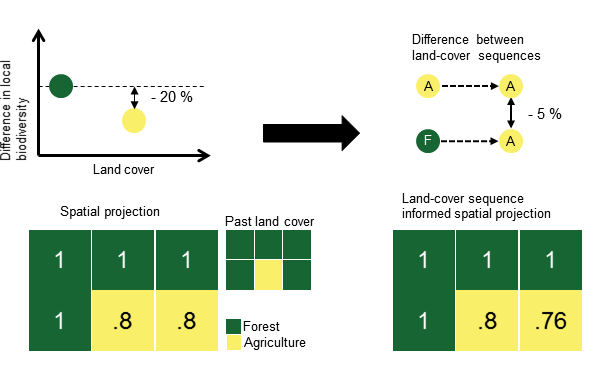
\includegraphics[width=1\textwidth]{chapter2/SI01}
\caption{ Flow chart showing all pre-processing steps of the analysis for both remote sensing and species assemblage data. Remote sensing data were derived from the MODIS Bidirectional reflectance distribution function (BRDF) MCD43A4 product (\href{https://tinyurl.com/mcd43a4-v006}{https://tinyurl.com/mcd43a4-v006}) and time series of the Enhanced Vegetation Index (EVI) were calculated for the analysis (see Methods). Species assemblage data originates from Projecting Responses of Ecological Diversity In Changing Terrestrial Systems project (PREDICTS, \href{http://www.predicts.org.uk/}{http://www.predicts.org.uk/}). MLE stands for the Maximum Linear Extent as defined by \citep{Hudson2016}.}
\label{SI02_01}
\end{figure}

% SI - Figure 2 Flowchart
\begin{figure}[h]
\centering
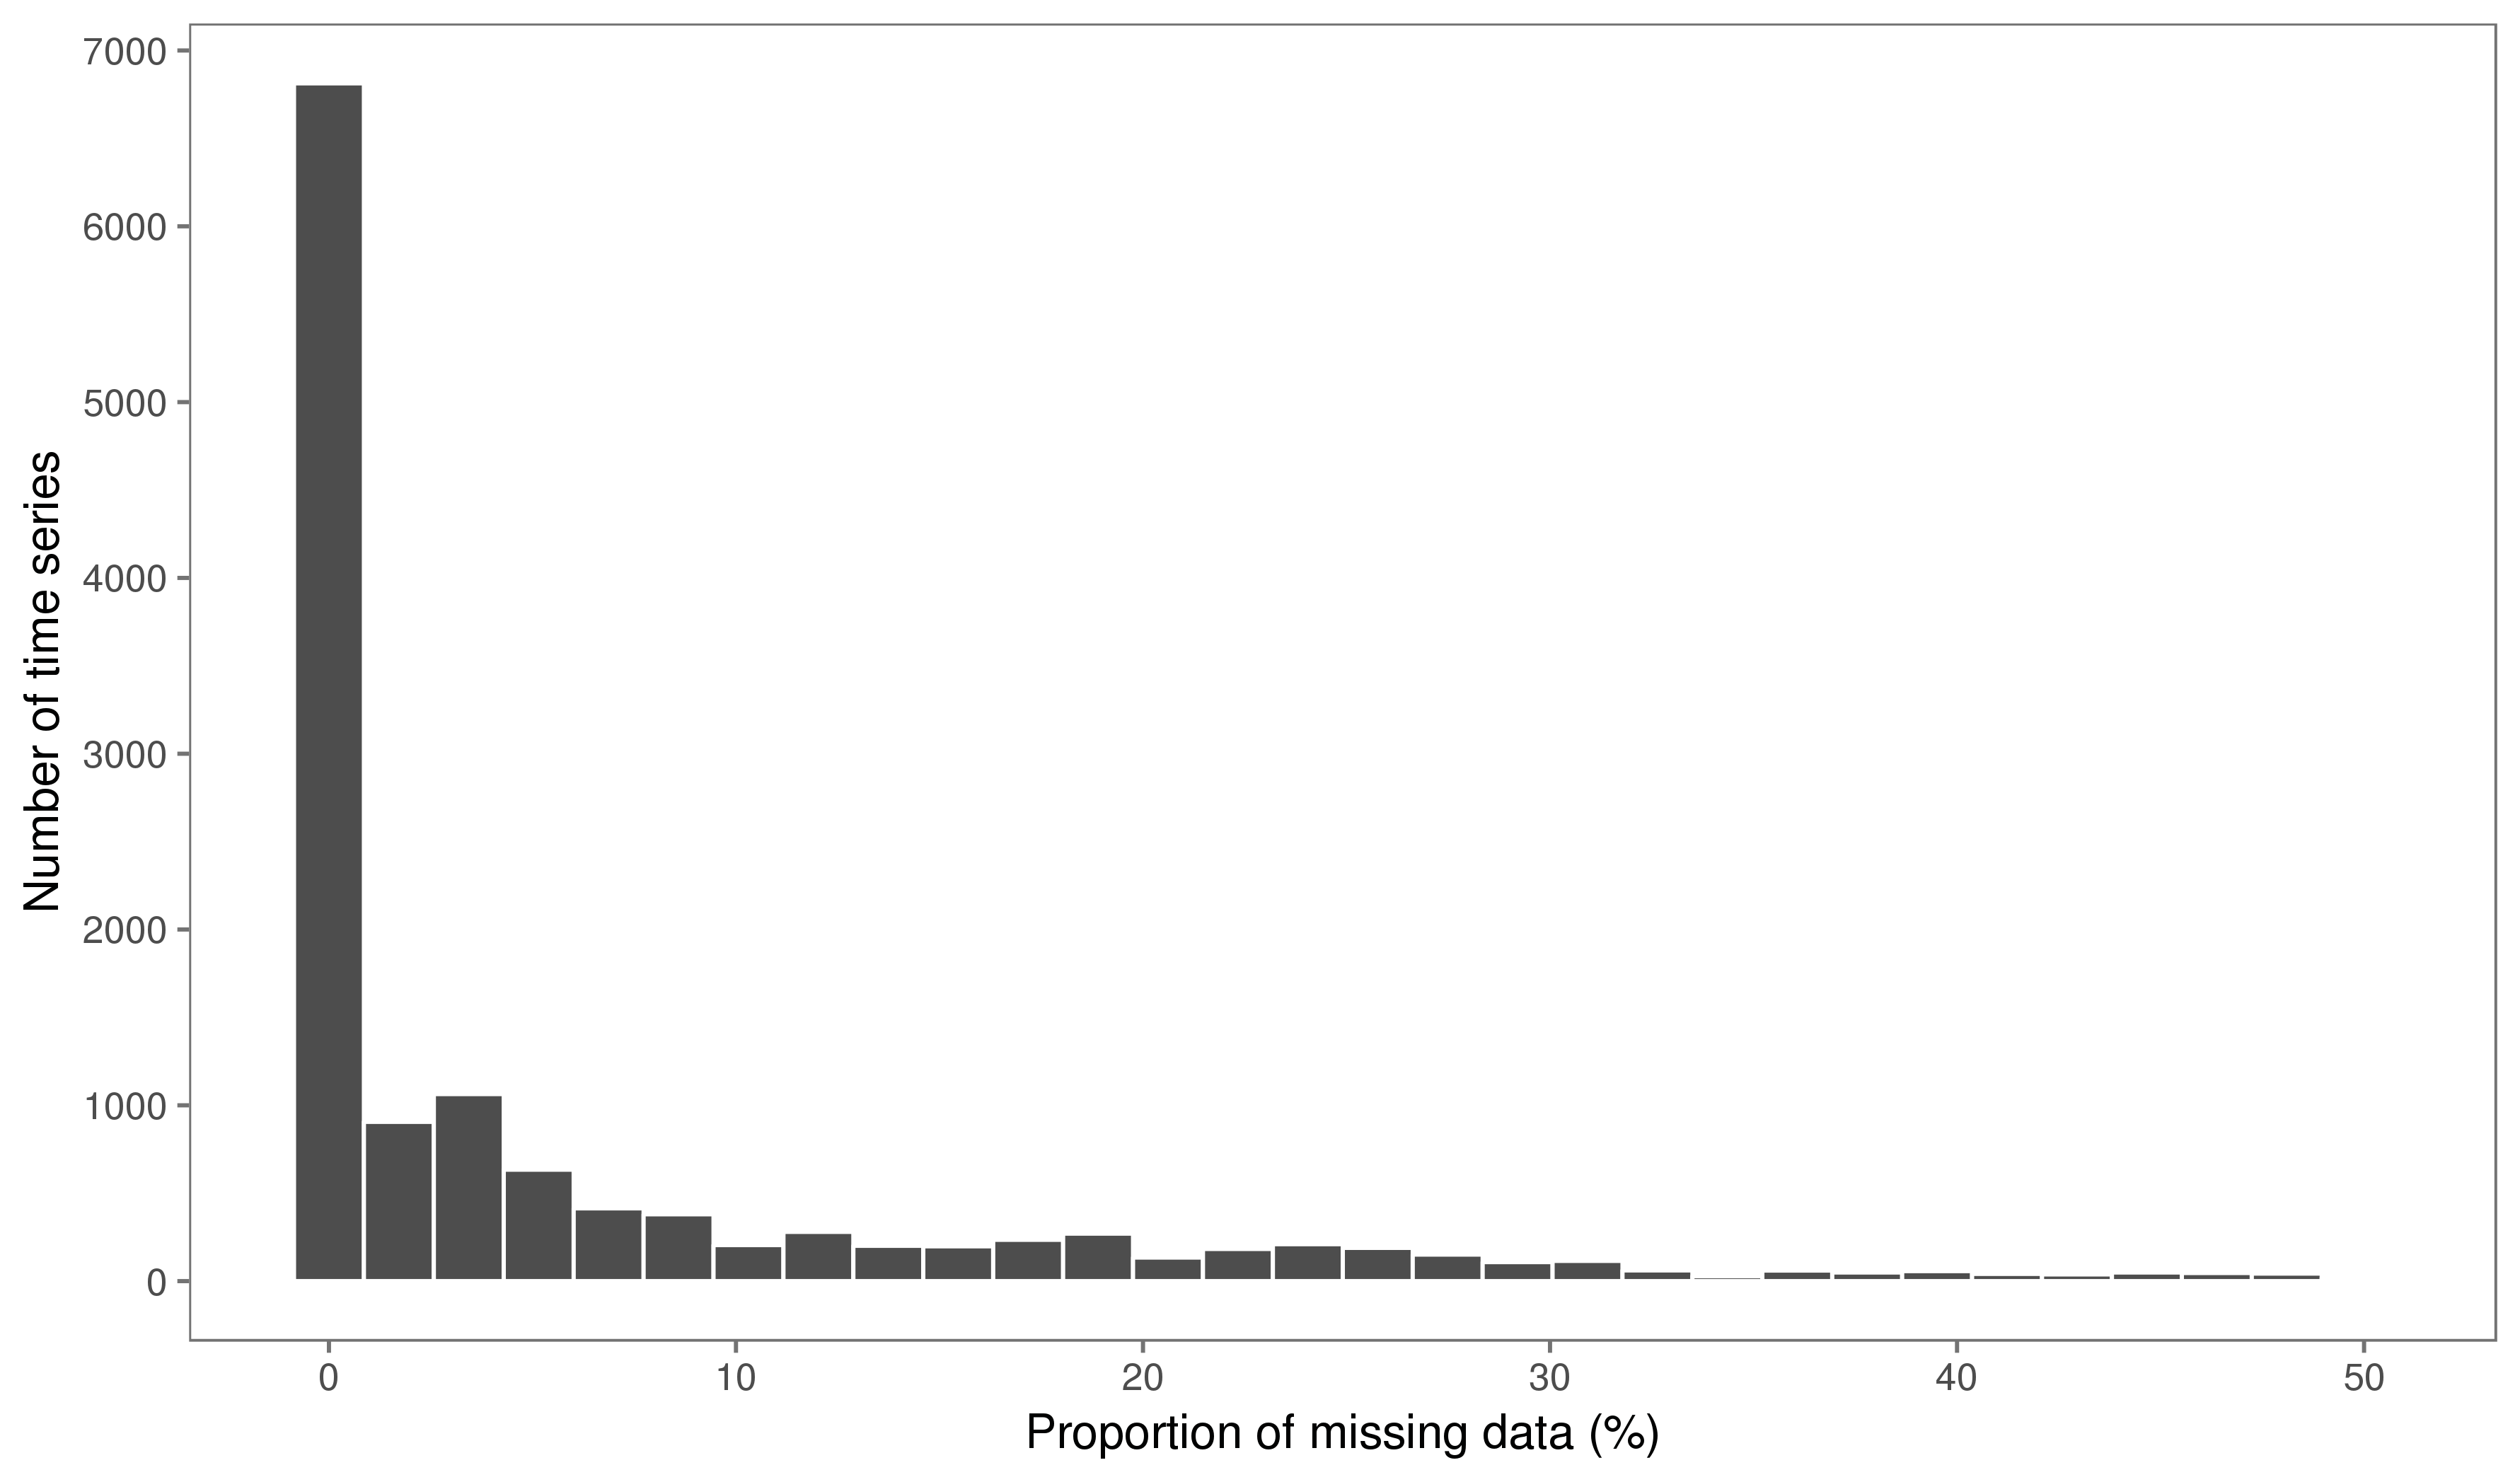
\includegraphics[width=1\textwidth]{chapter2/SI02}
\caption{ Distribution of proportion of missing data (not interpolated) across all time series used. }
\label{SI02_02}
\end{figure}

% SI - Figure 3 Pairwise permutation procedure
\begin{figure}[h]
\centering
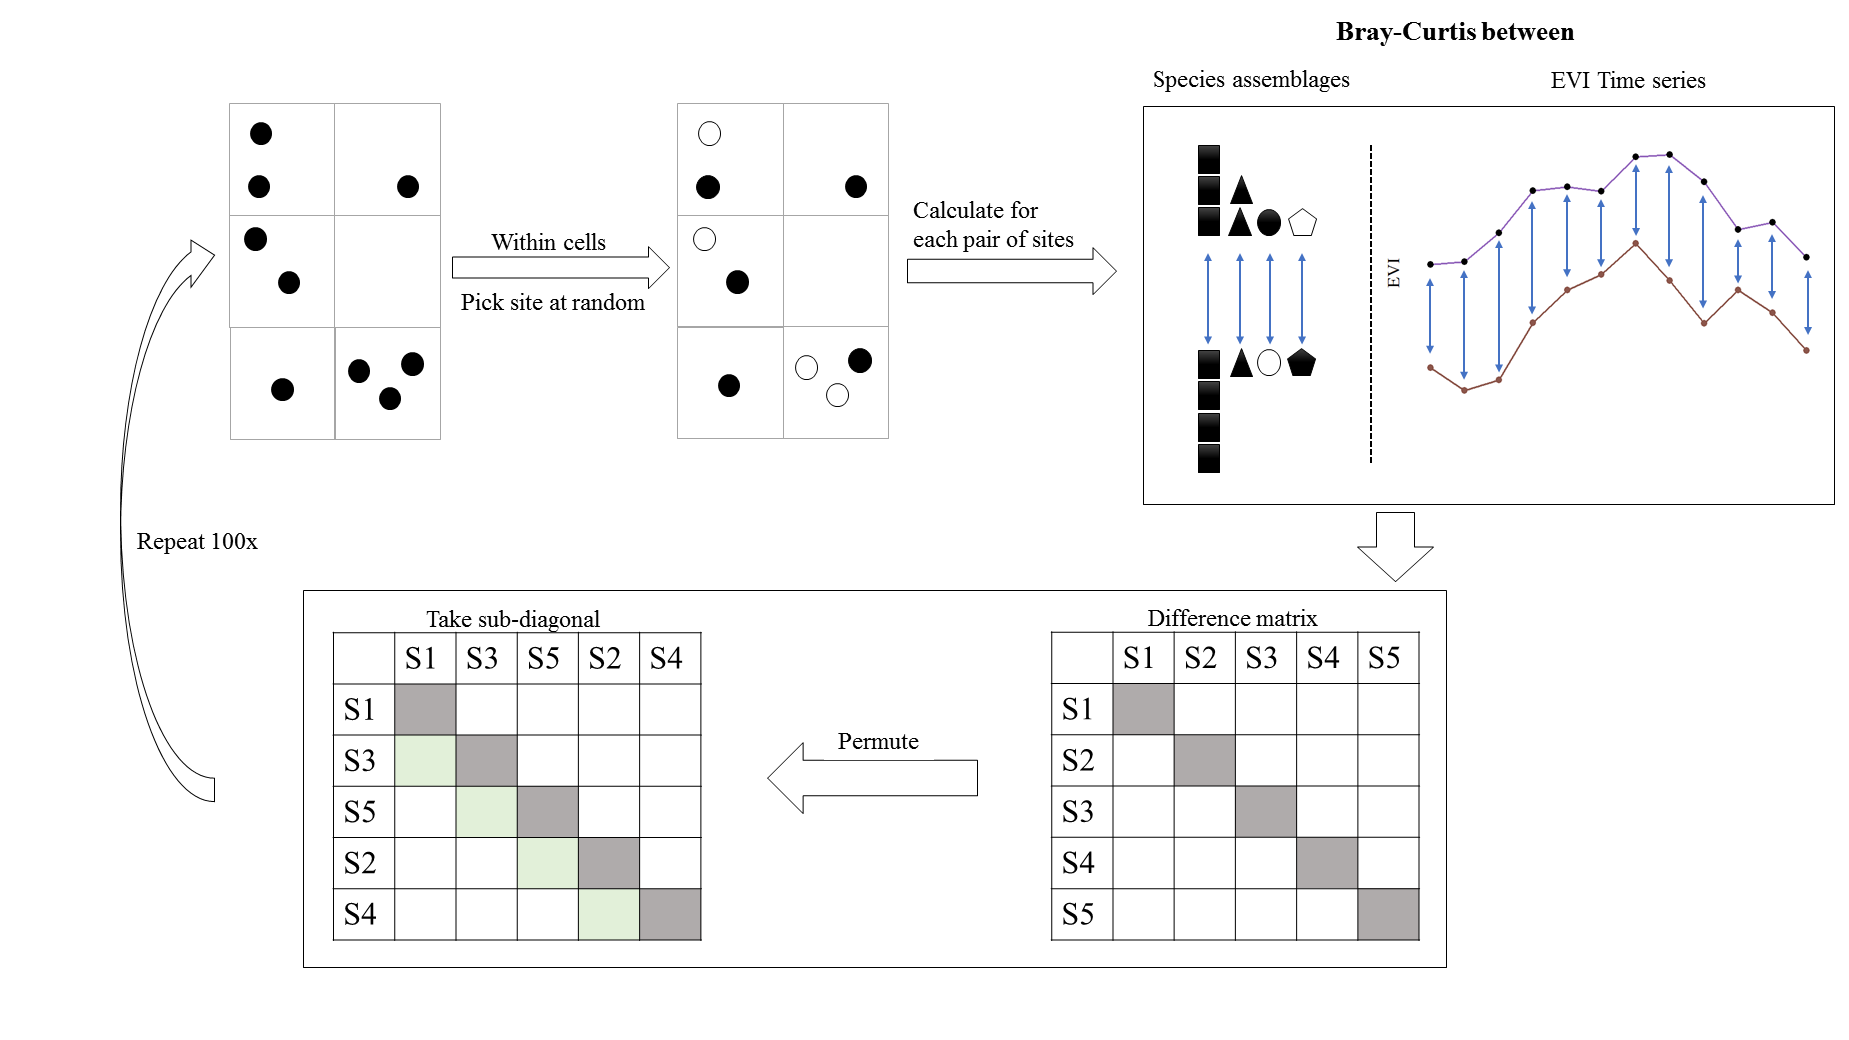
\includegraphics[width=1\textwidth]{chapter2/SI03}
\caption{ Diagram of how the permutations of mutually independent pairwise comparisons were generated. Black dots represent 9 theoretical sites of a study within MODIS grid cells of which one site (S1 – S5) per grid cell was randomly selected. We then calculated two dissimilarity matrices one matrix for the dissimilarity between species assemblages in that grid cell and all other grid cells within the study, and the other matrix for the dissimilarity between time series of the EVI of these grid cells.  For the time series, the Bray-Curtis index was calculated between the EVI values at each time step. For both species assemblages (symbols of varying number and shape) and EVI time series, the obtained dissimilarity matrix was permuted and the sub-diagonal taken for subsequent analysis. }
\label{SI02_03}
\end{figure}

% SI - Figure 4 Pairwise permutation procedure
\begin{figure}[h]
\centering
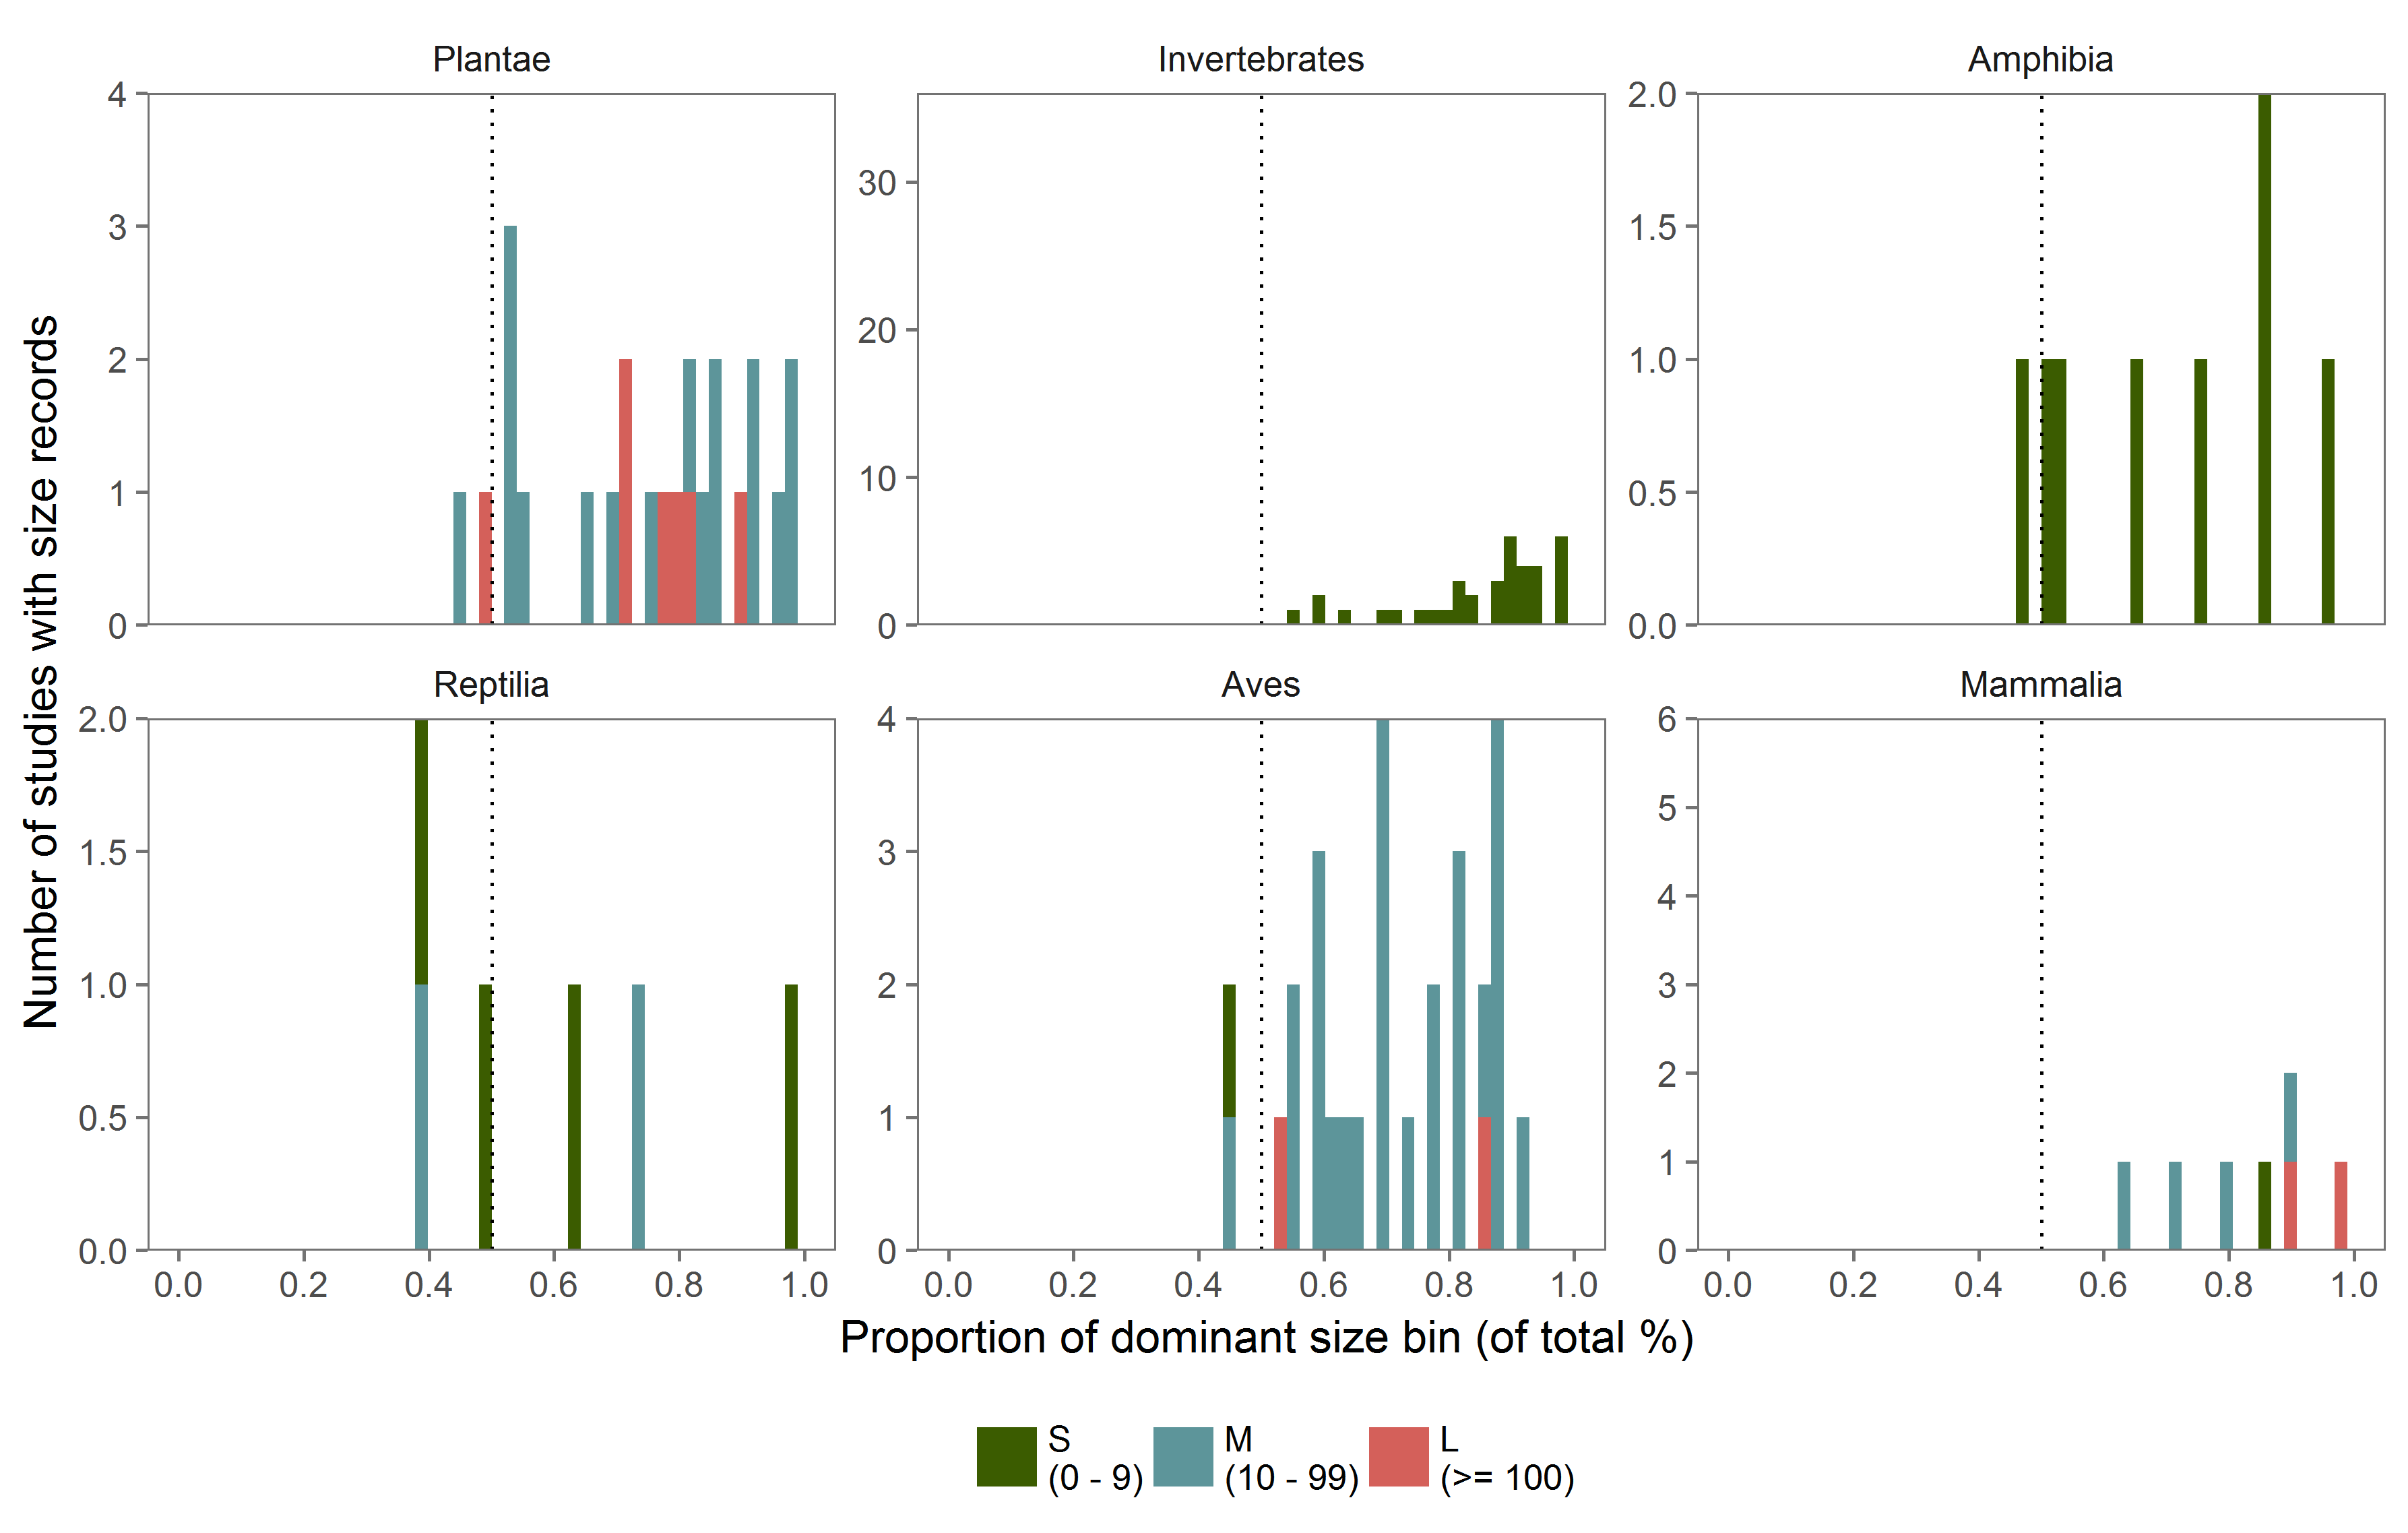
\includegraphics[width=1\textwidth]{chapter2/SI04}
\caption{ The proportion of species that contributed to a study being classified as either predominantly inhabited by small, medium or large species. The dotted line is a visual aid to assess simple majority (50\%) indicating whether a study classification is based on the majority of species within an assemblage. The y-axis shows the number of studies with similar proportions (note the difference in y-axis scale per taxonomic group). }
\label{SI02_04}
\end{figure}

% ------ %
% Regression table
\begin{sidewaystable}[h]
%\begin{table}[htb]
\centering
\caption{Averaged fixed effect, standard error (SE), marginal and conditional $R^2$ estimates as well as relative change in $R^2$ to current BC\textunderscript{EVI} of the overall average model (Figure \ref{F02_03}). N and N\textunderscript{sites} indicate the maximum number of studies and sites across permutations contributing to these estimates. }
\label{SIT02_01}
\begin{tabular}{llllllll}
\hline
Time Period & Slope & SE    & Marginal $R^{2}$ & Conditional $R^{2}$ & Relative difference $R^{2}$ & N   & N\textunderscript{sites} \\ \hline
yr\textunderscript{0}           & 0.289 & 0.064 & 0.012       & 0.464          & 0                      & 198 & 4053   \\
yr\textunderscript{1}           & 0.279 & 0.062 & 0.011       & 0.460          & -9.6                   & 198 & 4053   \\
yr\textunderscript{1-2}           & 0.299 & 0.065 & 0.012       & 0.462          & 0.4                    & 198 & 4053   \\
yr\textunderscript{1-3}           & 0.316 & 0.067 & 0.013       & 0.462          & 9.1                    & 198 & 4053   \\
yr\textunderscript{1-4}           & 0.323 & 0.069 & 0.013       & 0.463          & 11.2                   & 198 & 4053   \\
yr\textunderscript{1-5}           & 0.334 & 0.071 & 0.014       & 0.463          & 16.7                   & 198 & 4053   \\ \hline
\end{tabular}
\end{sidewaystable}
%\end{table}
% ------ %

% SI - Figure 5 Plot per taxonomic group
\begin{figure}[h]
\centering
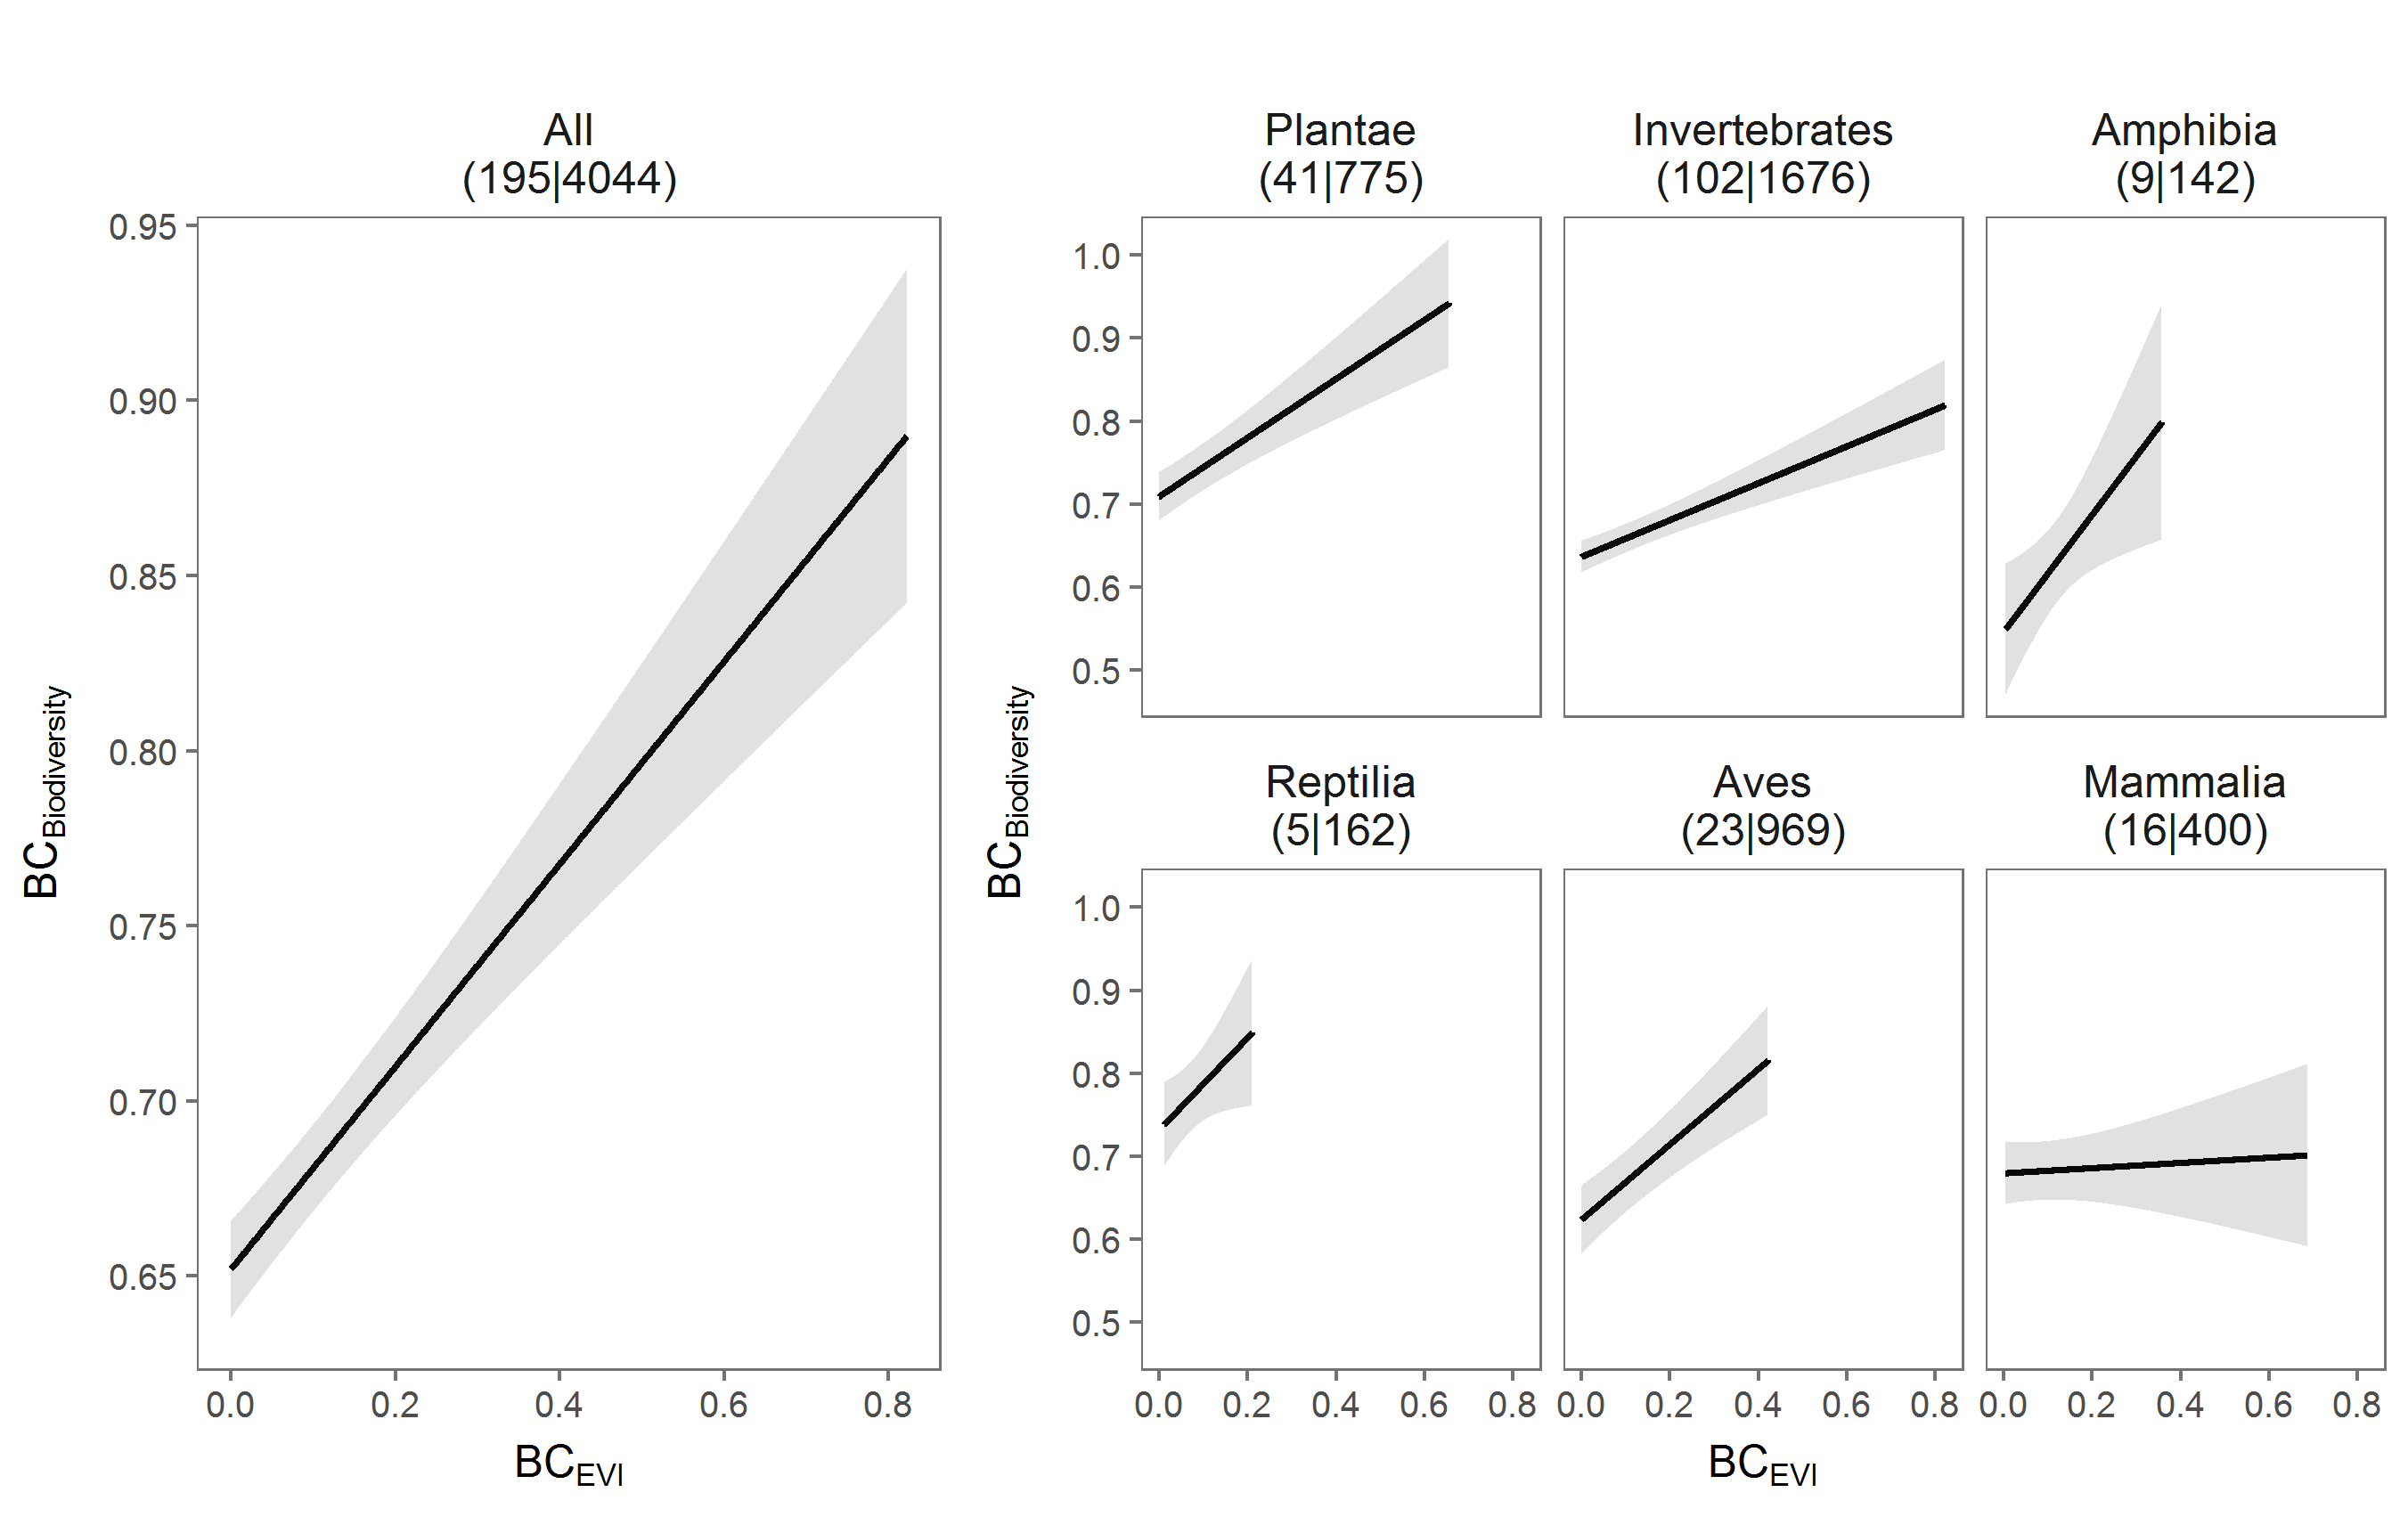
\includegraphics[width=1\textwidth]{chapter2/SI05}
\caption{ Effect of differences in current BC\textunderscript{EVI} in the first year before biodiversity sampling against their pairwise differences in species assemblages (BC\textunderscript{Biodiversity}). The number of studies and contributing sites (N|N\textunderscript{Sites}) is indicated for each taxonomic group. }
\label{SI02_05}
\end{figure}

% SI - Figure 6 Simulation
\begin{figure}[h]
\centering
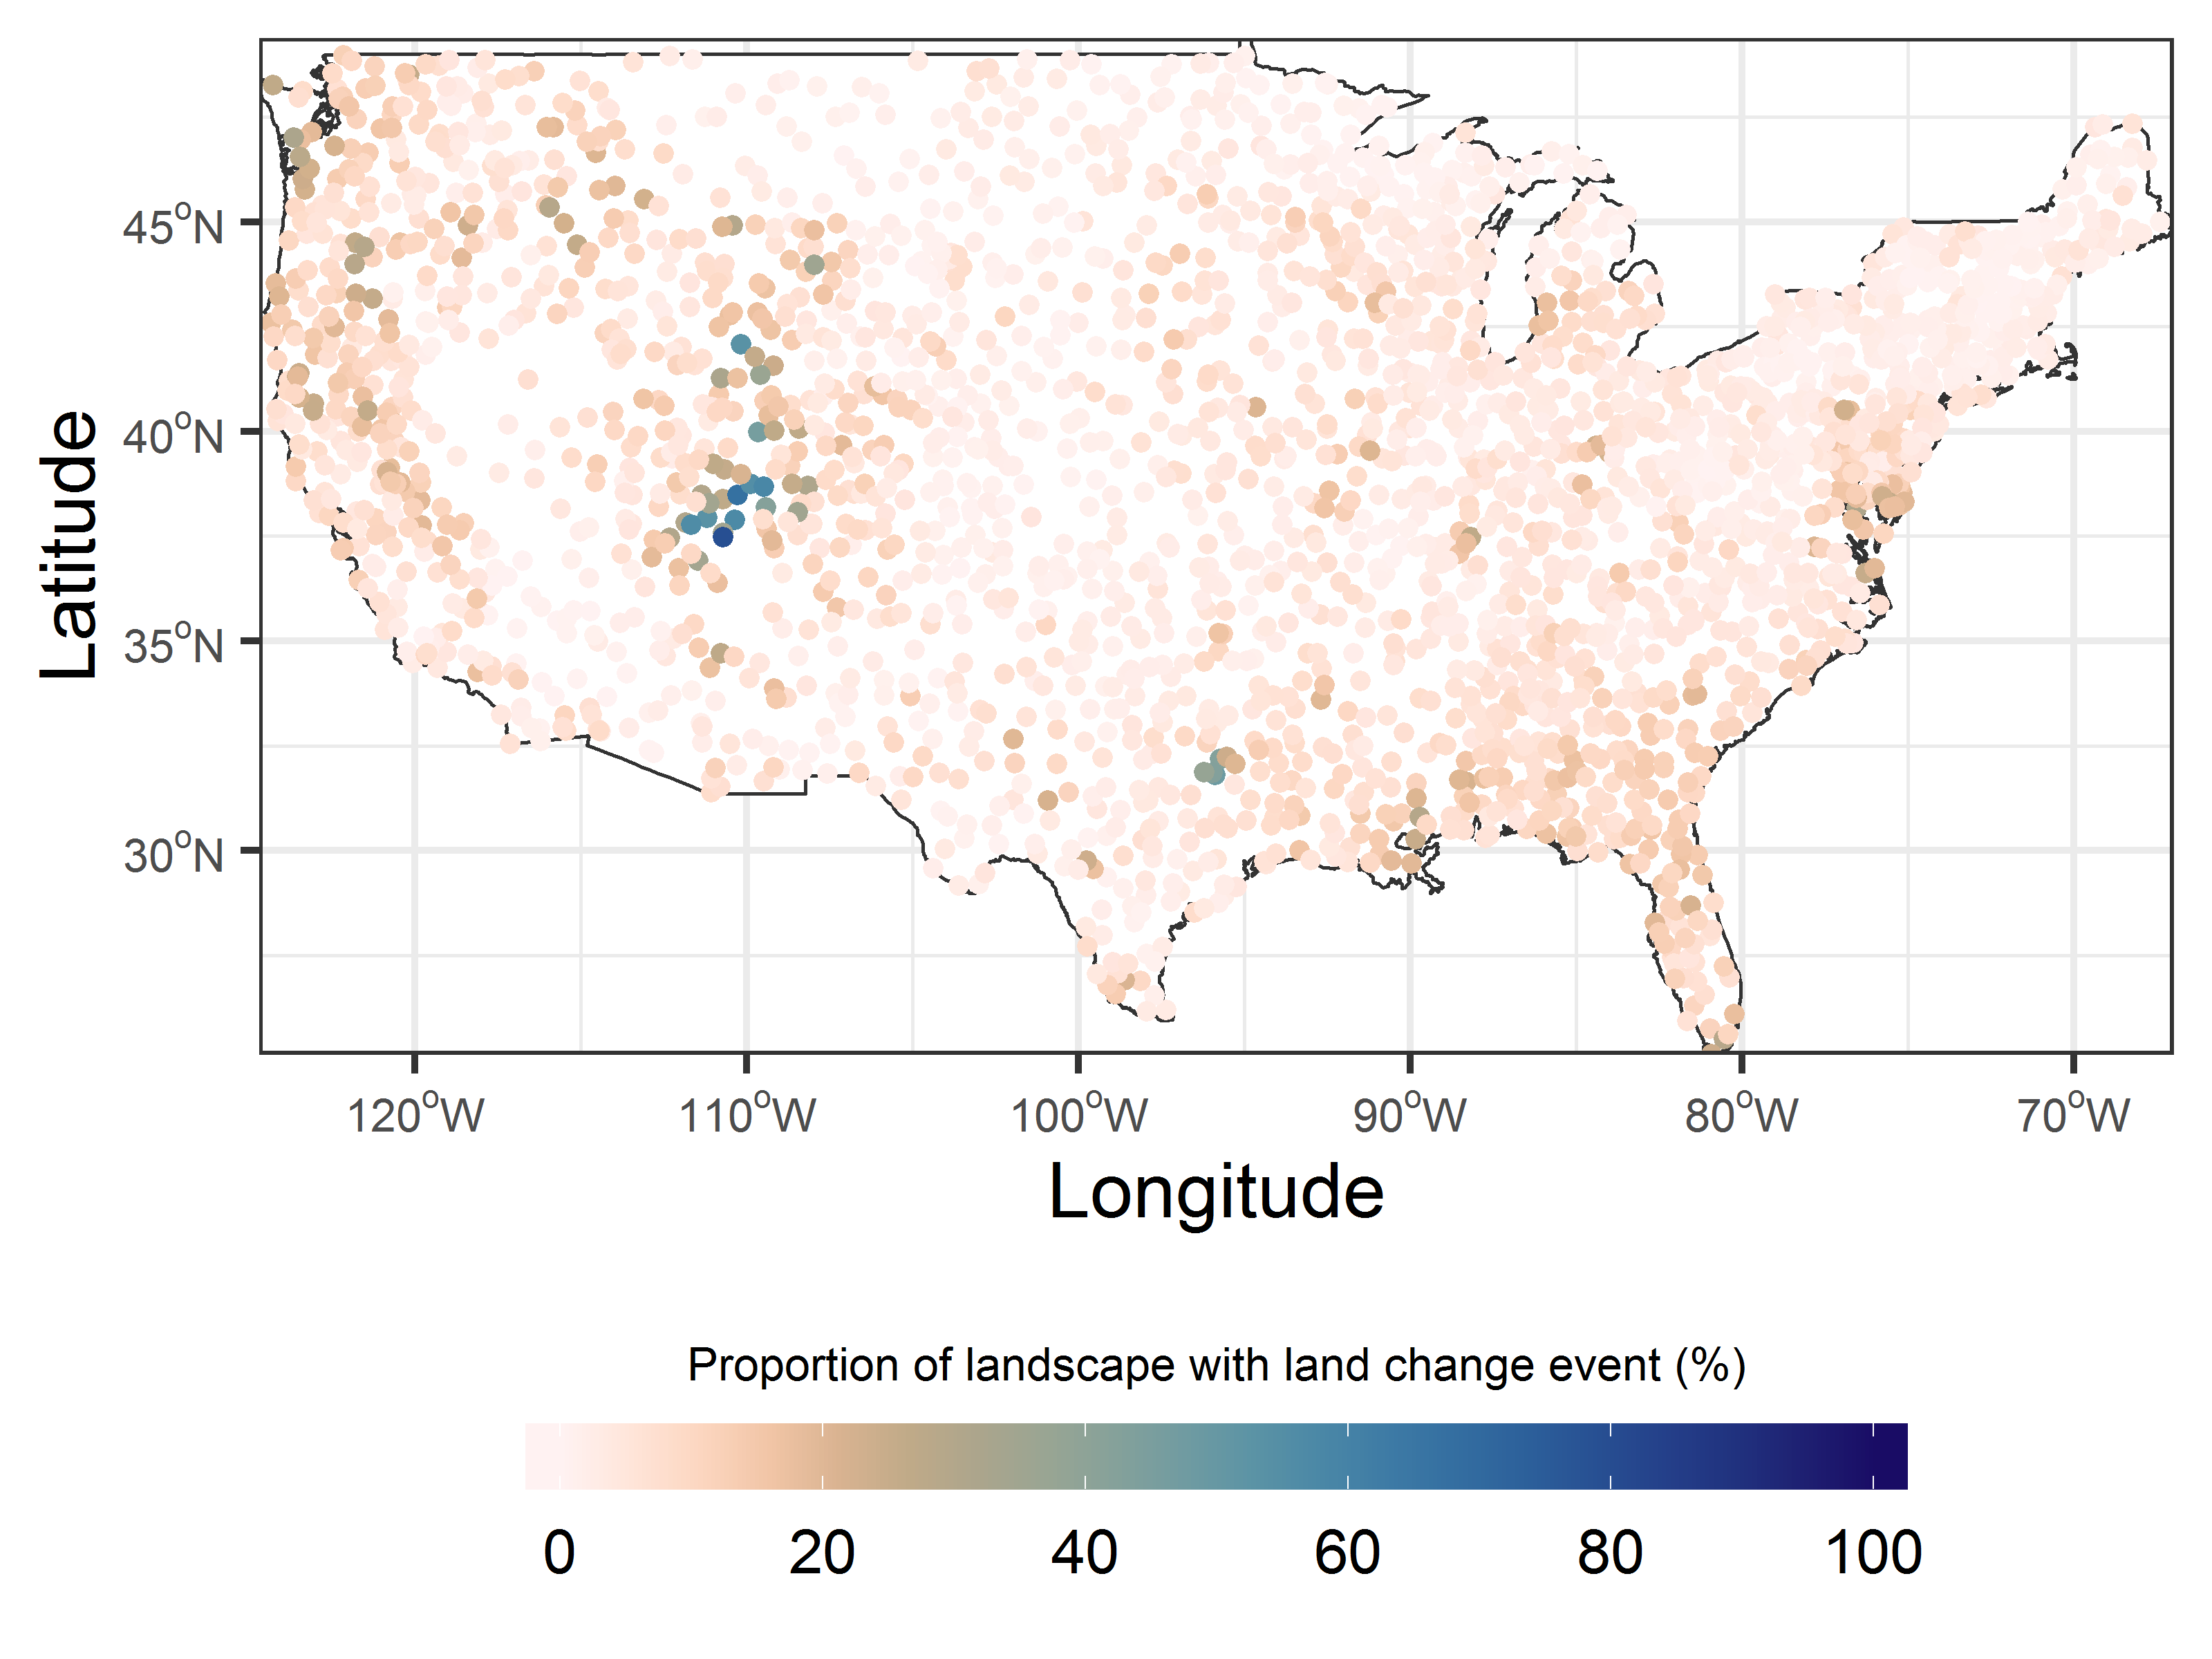
\includegraphics[width=1\textwidth]{chapter2/SI06}
\caption{ Simulation of how the Bray-Curtis index (BC\textunderscript{EVI}) between two time series changes with increasing time series length. Calculated on pairs of randomly generated time series for each past period. Vertical dotted lines indicate periods of full past years of theoretical possible MODIS measurements (46 each, increasing from 46 initially for current BC\textunderscript{EVI}). There is no overall bias that the Bray-Curtis index increases with time series length (blue line shows a linear regression fit; $\beta$ < 0.0001, df = 229, p = 0.44).}
\label{SI02_06}
\end{figure}

% SI - Figure 7 Spatial autocorrelation
\begin{figure}[h]
\centering
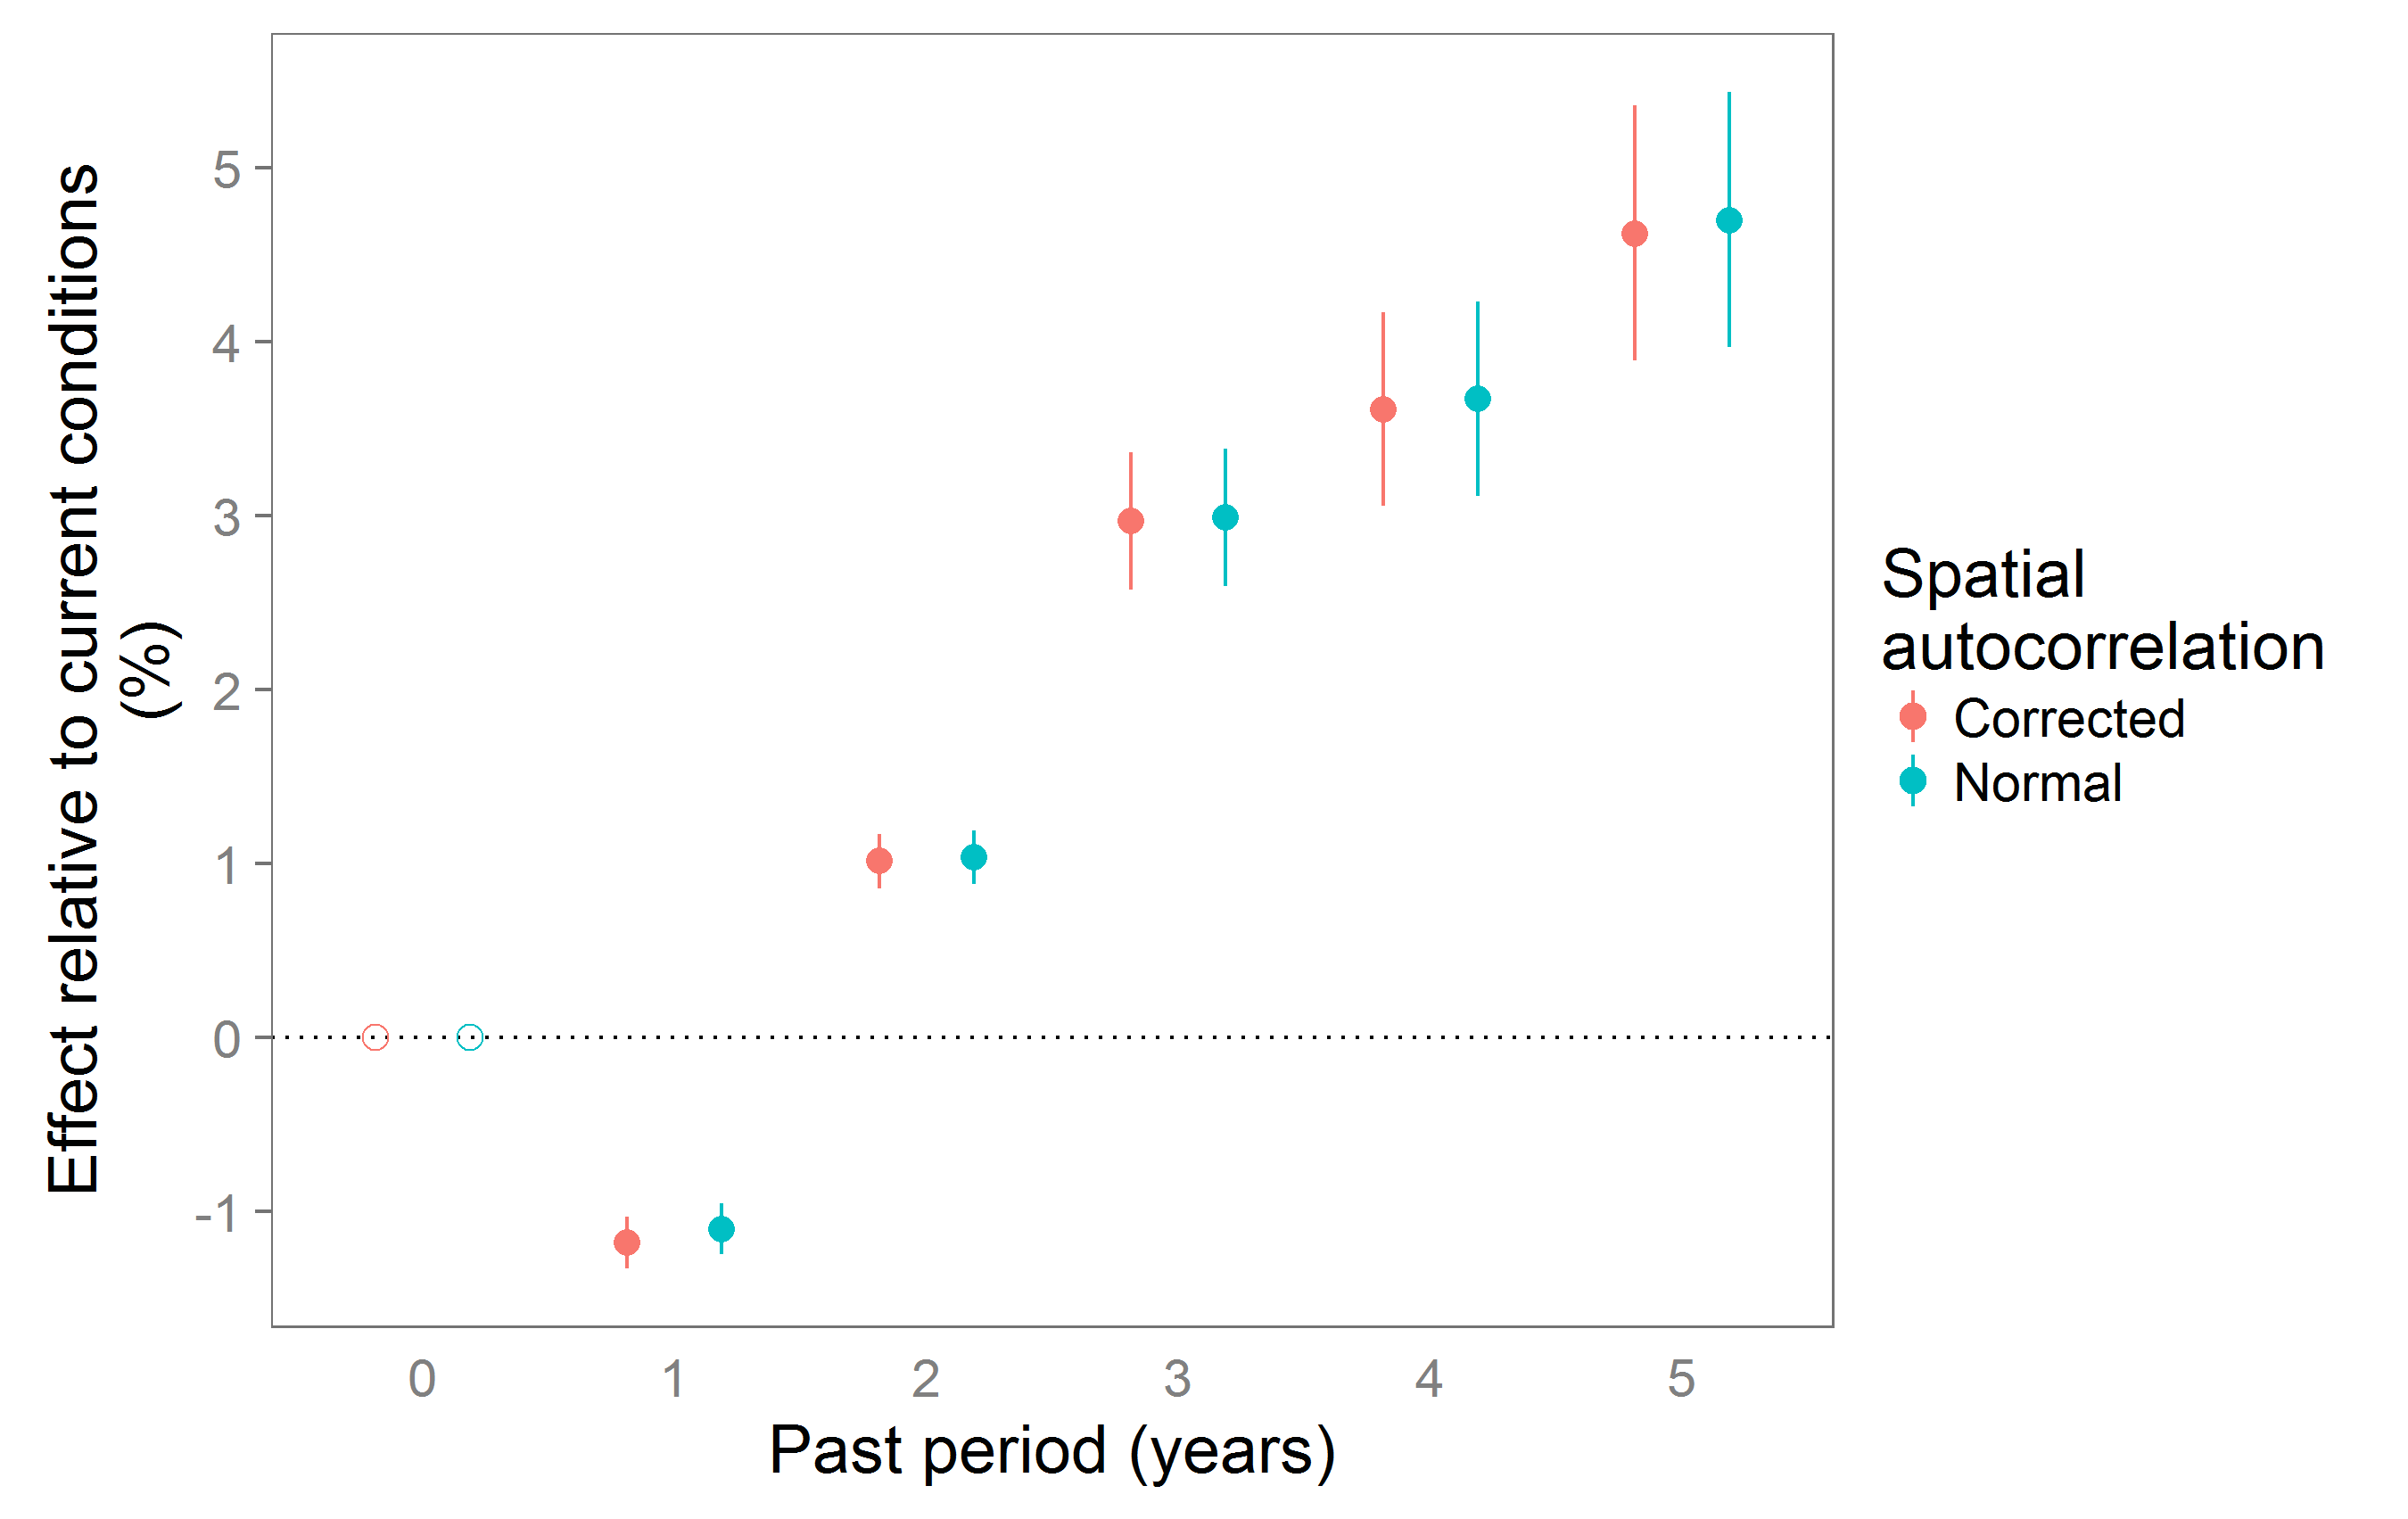
\includegraphics[width=1\textwidth]{chapter2/SI07}
\caption{ Difference in overall fit if studies with significant residual correlation with spatial distance (N=1) are removed. X-axis shows the current (0) and past periods (yr\textunderscript{1-5}), while the y-axis shows the difference in effect relative to the effect of current BC\textunderscript{EVI}.}
\label{SI02_07}
\end{figure}

% SI - Figure 8 Any biases
\begin{figure}[h]
\centering
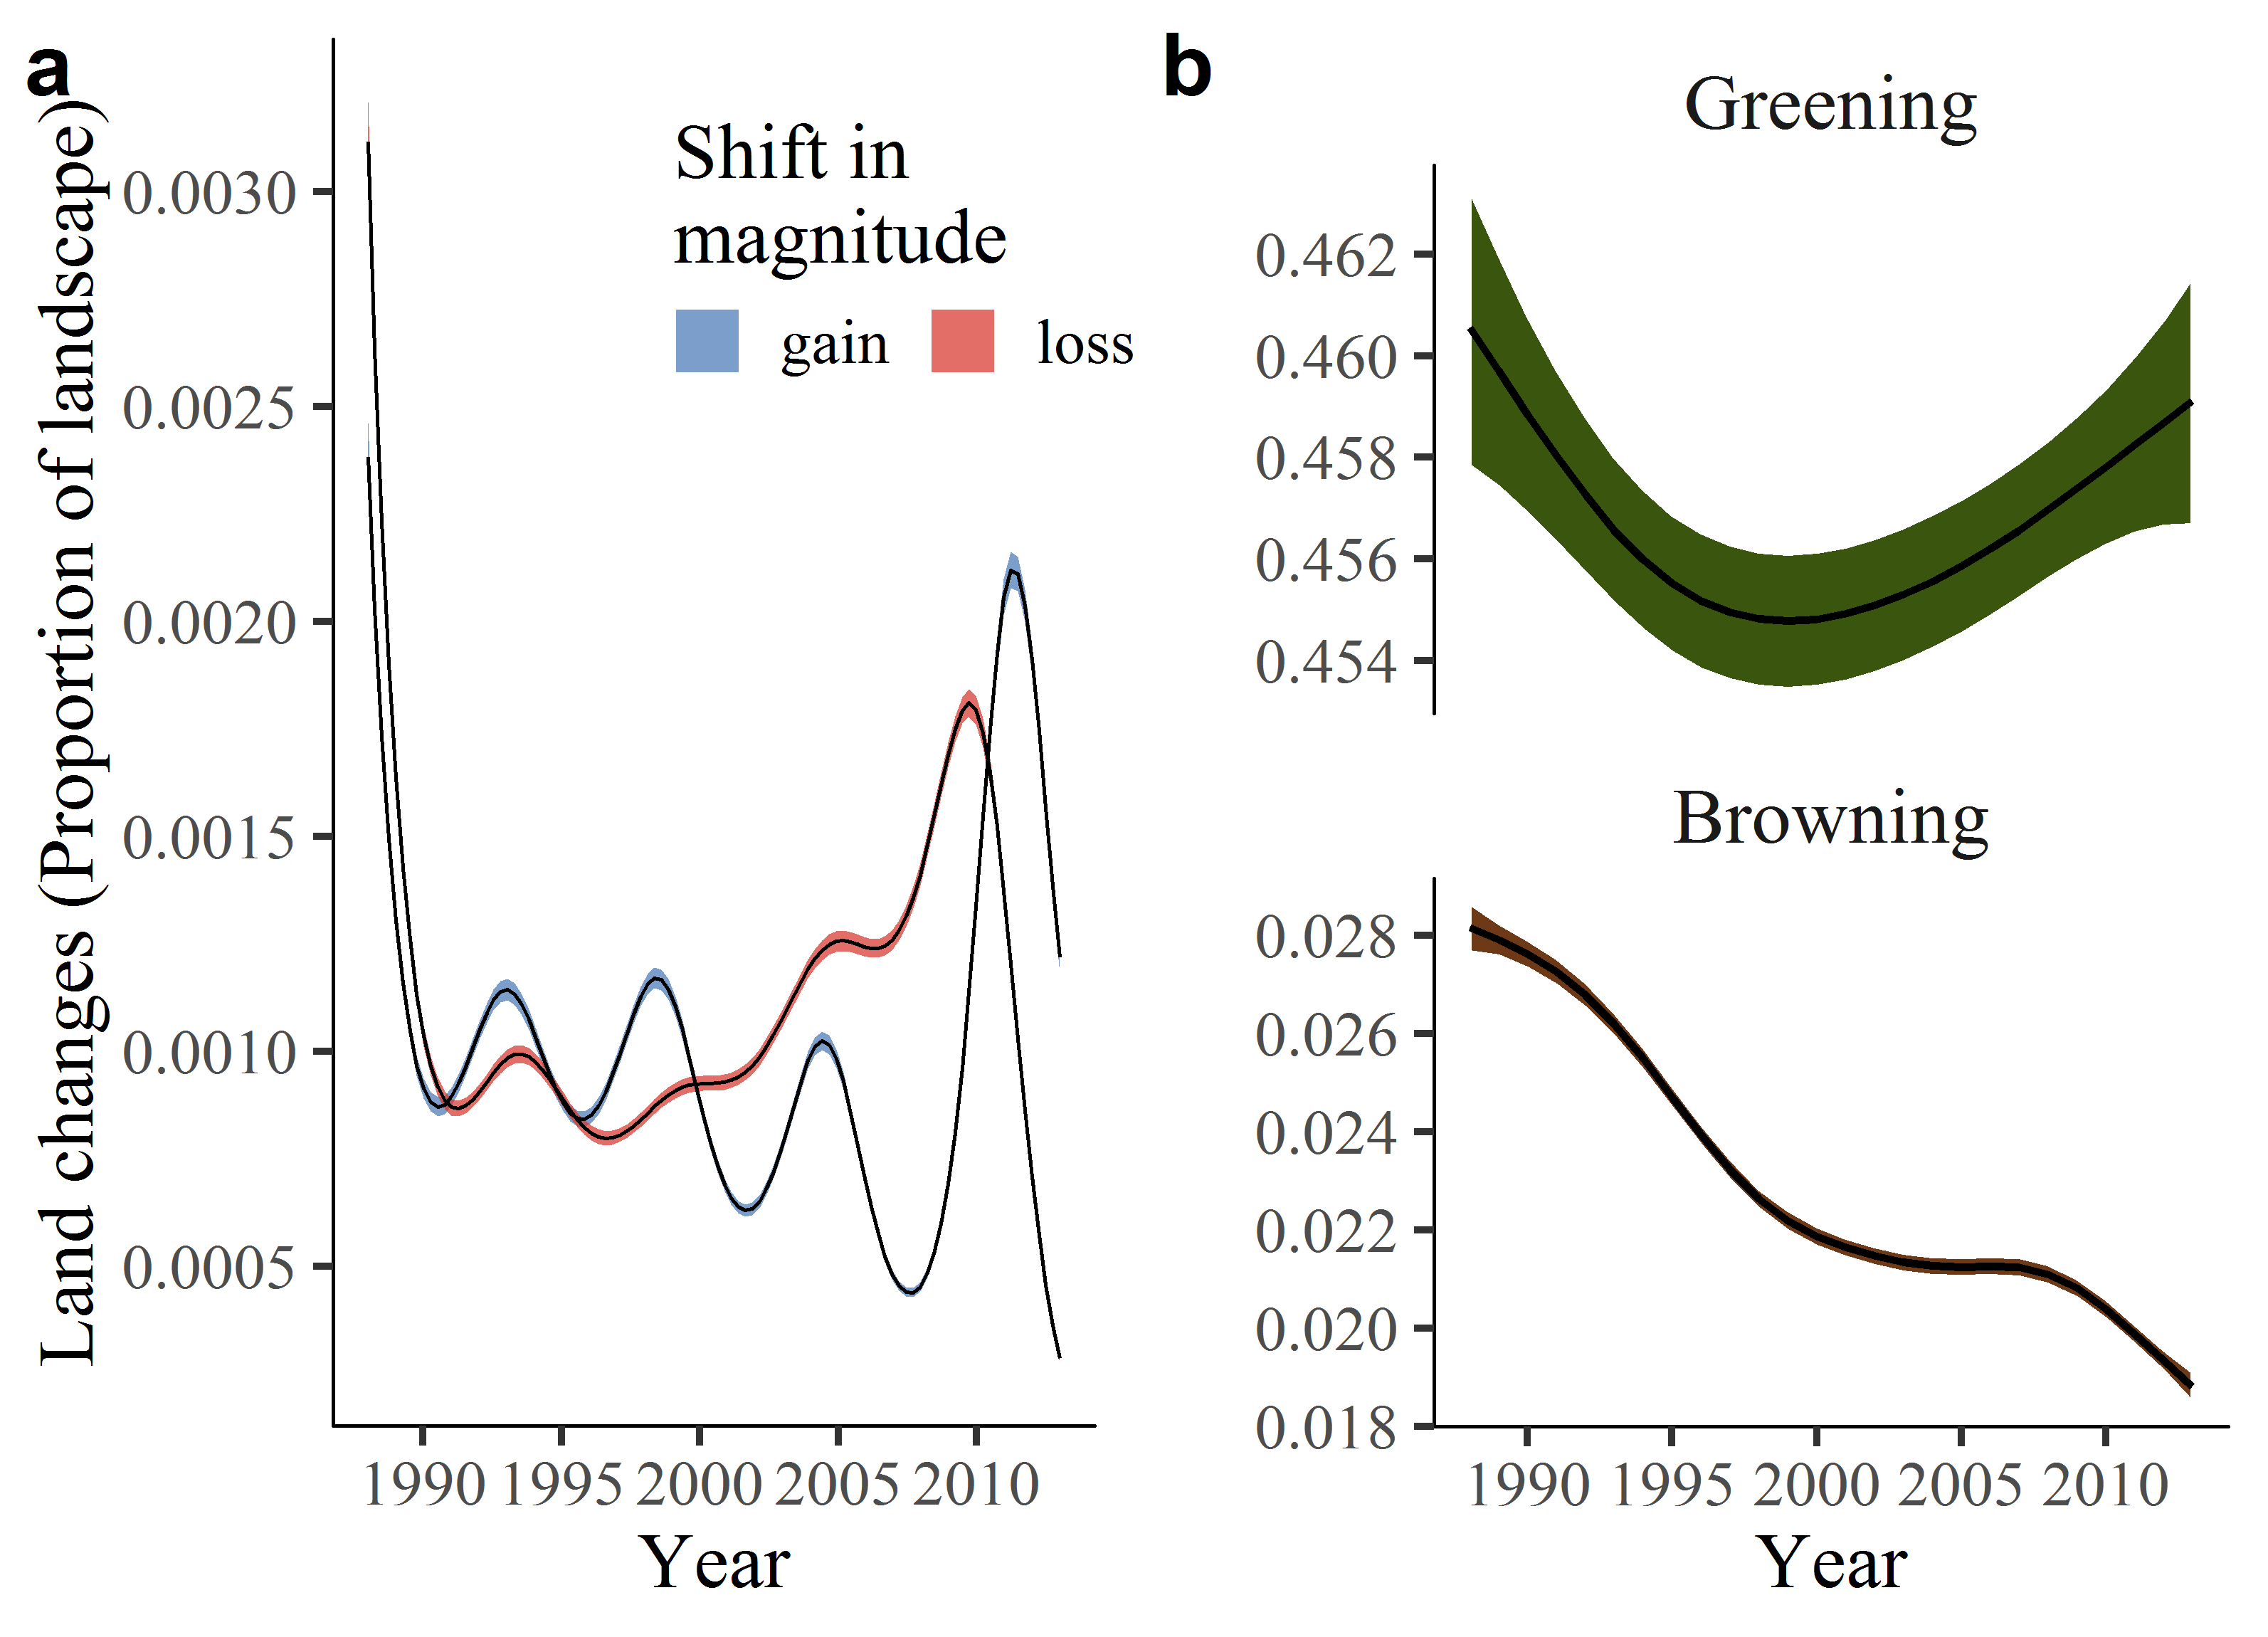
\includegraphics[width=1\textwidth]{chapter2/SI08}
\caption{ Investigation of potential broad-scale biases of the full model coefficients (5-year period). There is no bias in the permuted model effects with regards to (\textbf{a}) year of biodiversity sampling, (\textbf{b}) spatial scale of sampling, (\textbf{c}) average sampling duration, or (\textbf{d}) average latitude of study (grey shading indicates tropic belt).}
\label{SI02_08}
\end{figure}

% SI - Figure 9 Using another metric
\begin{figure}[h]
\centering
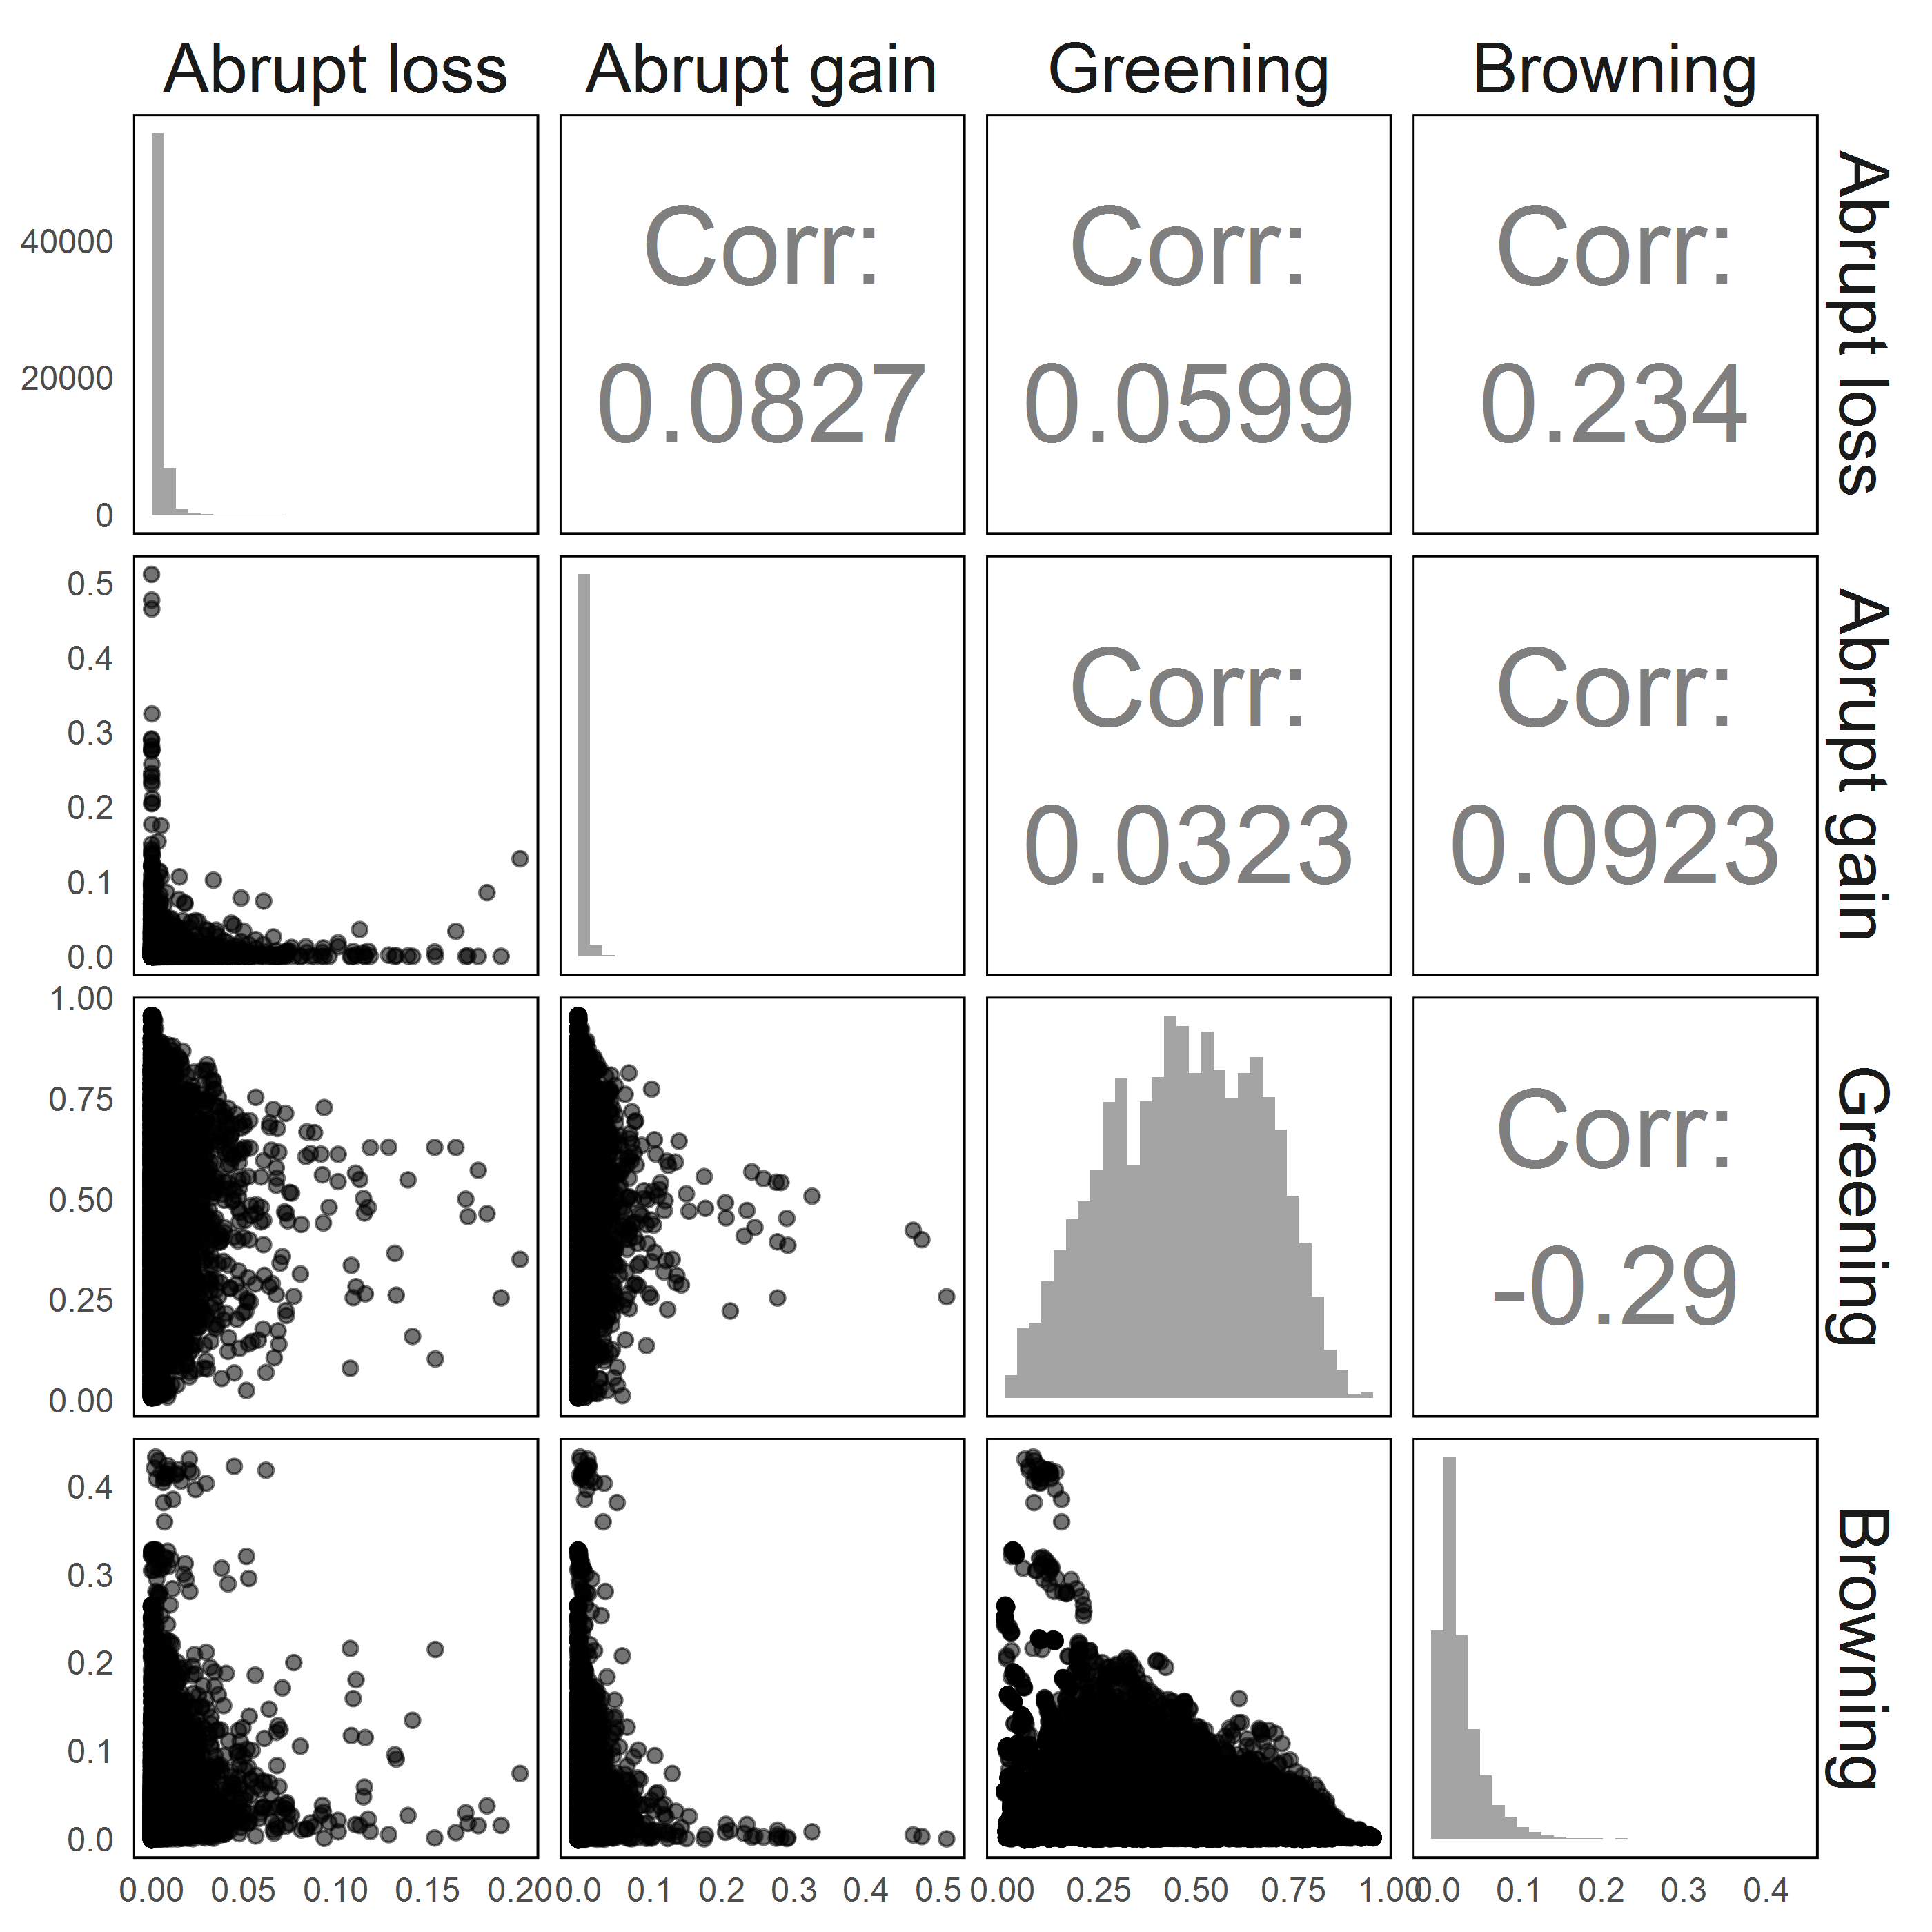
\includegraphics[width=1\textwidth]{chapter2/SI09}
\caption{ Overall influence of past periods of BC\textunderscript{EVI} on species assemblage composition as in Figure \ref{F02_03}, however shown for both Bray-Curtis index and as alternative the S\o rensen index. Axis labels as in Figure \ref{F02_03}.}
\label{SI02_09}
\end{figure}
